\section{Introdução e Justificativas}\label{Intro}


%=============================================================================
% 							INTRODUÇÃO
%=============================================================================

%GFC E QUESTIONAMENTO DO INVESTIMENTO COMO CAUSA CAUSANS
Ainda que os impactos sócio-econômicos da Crise Financeira Global (CFG) são imensuráveis, algumas mudanças sobre a teoria econômica já podem ser tateadas. Se, por um lado, abalou a macroeconomia ortodoxa ao ponto da política fiscal estar sendo repensada, por outro, redirecionou algumas pautas na heterodoxia. Distribuição e desigualdade, temas tão caros a esta última tradição, ganharam novo fôlego \cites{carvalho_personal_2016}{ederer_will_2019} enquanto parte da literatura passou a destacar o consumo como um dos possíveis motores de crescimento \cite{brochier_macroeconomics_2017}. Paralelamente, verificou-se um crescente interesse nas implicações macroeconômicas do investimento residencial\footnote{E isso é verificado até na literatura ortodoxa. Inspecionando modelos DSGE que incluem investimento residencial, \textcite{iacoviello_housing_2010} conclui que um melhor entendimento dos impactos deste gasto se faz necessária para a compreensão das flutuações macroeconômicas. } \cite{fiebiger_semi-autonomous_2018}. Desse modo, foi identificado que umas das consequências da CFG é a reconsideração do investimento (das firmas) ser ou não  ``a causa das causas''.

Neste ponto, cabe mencionar o ineditismo de \textcite{green_follow_1997} e \textcite{leamer_housing_2007} --- e revisitado em \textcite{leamer_housing_2015} e por \textcite{fiebiger_trend_2017} --- ao lançar luz sobre a importância do investimento residencial na determinação dos ciclos econômicos em todo o pós-guerra. Ao avaliar o caso norte-americano, \textcite{green_follow_1997} conclui que o investimento residencial possui uma capacidade preditiva maior que o investimento das firmas, mas que isso não implica no estabelecimento de uma relação causal. Na tentativa de compreender tais resultados, afirma:

\begin{quote}
	
	[P]\textit{erhaps residential investiment, like stock prices and interest rates, is a good predictor of GDP because it is a series that reflects \textbf{foward looking behavior}. Presumably households will not increase their expenditures on housing unless they expect to prosper in the future. Building a house is a natural mechanism for doing this. Thus, the series can do a good job of predicting GDP without necessarily causing GDP.}
	\cite[p.~267, grifos adicionados]{green_follow_1997}
\end{quote}
\textcite{leamer_housing_2007}, por sua vez, destaca a capacidade preditiva e relação causal  deste gasto com o PIB\footnote{Recentemente, \textcite{huang_is_2018} testam ambas as hipóteses aventadas por Leamer  (predição e causalidade) para os países da OCDE e concluem que o investimento residencial não é um mero canal de transmissão da política monetária enquanto os resultados sobre a relação de causalidade não são conclusivos para todos os países da OCDE --- mas presente nos países do G7 --- dada heterogeneidade institucional observada.}. Sucintamente, afirma que a construção de novos imóveis permite, via aumento das linhas de crédito, um maior consumo de bens duráveis e, portanto, o ciclo econômico americano pode ser configurado como um \textit{consumer cycle} e não como um \textit{business cycle}. Em outras palavras, por ser  uma das formas de riqueza mais comuns entre as famílias norte-americanas, o investimento residencial servia de colateral para tomada de crédito \cite{teixeira_uma_2011}. A forma de ``realizar'' o ganho de capital com a bolha imobiliária que ocorreu no período, sem precisar liquidar os imóveis, era justamente ampliando o endividamento à medida que este colateral (\textit{i.e.} imóveis) aumentava de valor \cite{teixeira_crescimento_2015}. 
%MAIS REFERÊNCIAS EUA?

Uma análise complementar é a da  ``hipotecarização'' desenvolvida por \textcite{jorda_great_2014} que destaca a crescente participação das hipotecas nos balanços patrimoniais dos bancos\footnote{\textcite{jorda_great_2014} também destacam que o crédito hipotecário era concedido fora do sistema bancário até os 1900 e isso dificulta a estimação dos dados.} (ver gráfico \ref{GraficoJorda}). A partir do desenvolvimento de uma base de dados que contém os subcomponentes dos empréstimos dos bancos desde 1880, os autores destacam que os empréstimos às famílias têm aumentado a uma velocidade superior ao valor de seus ativos e, portanto, verifica-se uma maior alavancagem --- logo, maior fragilidade financeira das famílias --- apesar do aumento do preço dos imóveis. Portanto, a compreensão do papel das hipotecas no sistema bancário bem como do investimento residencial para o crescimento se justifica pelos impactos reais e financeiros sobre o ciclo econômico: 

\begin{quote}
	\textit{To a large extent the core business model of banks in advanced economies today resembles that of real estate funds: banks are borrowing (short) from the public and capital markets to invest (long) into assets linked to real estate.} [...] \textit{looking more deeply at the composition of bank credit, it becomes clear that the rapid growth of \textbf{mortgage lending} to households has been the \textbf{driving force} behind this remarkable change in the composition of banks’ balance sheets} \cite[p.~2, grifos adicionados]{jorda_great_2014}
\end{quote}

\begin{figure}
	\centering
	\caption{Participação do empréstimo imobiliário no total do balanço patrimonial dos bancos (1880-2016)}
	\label{GraficoJorda}
	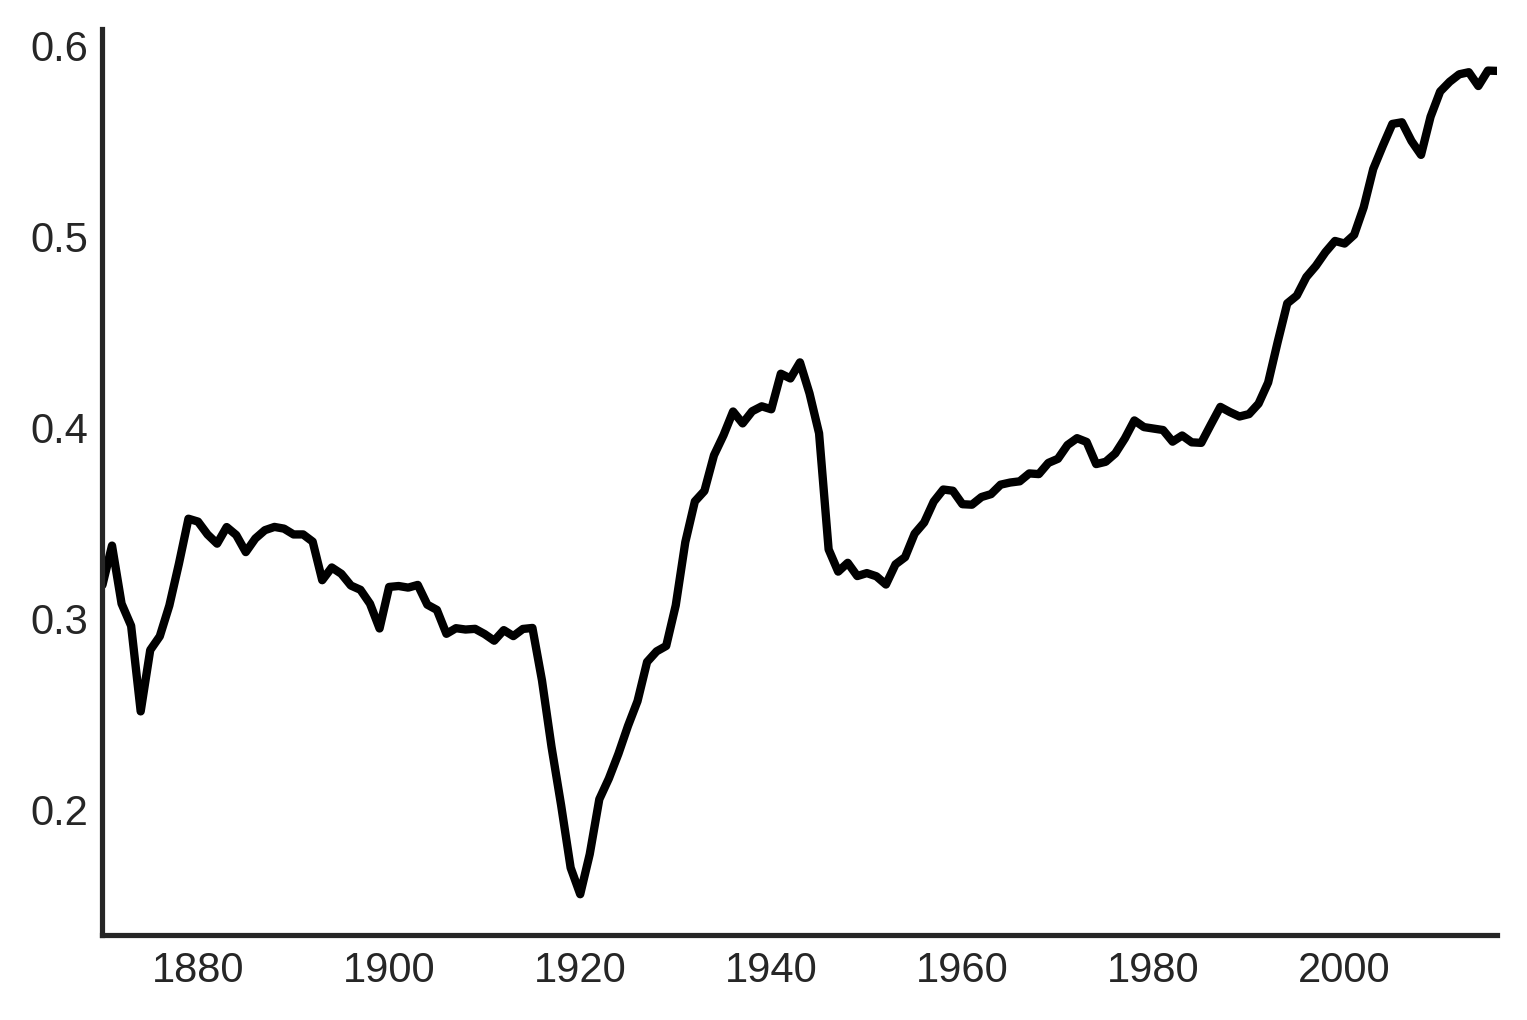
\includegraphics[width=.7\textwidth]{Jorda_Mean.png}
	\caption*{\textbf{Fonte:} \textcite[p.~10]{jorda_great_2014}}
\end{figure}


Recentemente, parte da literatura econométrica também tem lançado luz sobre a importância do investimento residencial para o ciclo econômico\footnote{Além da importância do investimento residencial para a dinâmica econômica, cabe pontuar a relevância da taxa de aquisição de imóveis na determinação do endividamento das famílias e, portanto, destacar a importância de se estudar o tema \cite{schwartz_politics_2009}.
}. \textcite{alvarez_does_2010}, por exemplo, concluem que tal tipo de investimento antecede o ciclo econômico para o caso espanhol e resultados semelhantes podem ser encontrados para França, Espanha  e Itália enquanto o caso alemão apresenta uma dinâmica distinta \cites{ferrara_cyclical_2010}{ferrara_common_2010}. 
Outros estudos empíricos, por sua vez, têm enfatizado o efeito riqueza --- via valorização dos imóveis --- sobre o consumo e indicam tais canais de transmissão são mais incidentes, em ordem, sobre Estados Unidos e Grã Bretanha e mais brandos no caso francês e alemão \cites{sastre_assessment_2010}{chauvin_wealth_2010}{bassanetti_effects_2010}{arrondel_housing_2010}.

A pluralidade de resultados reportada acima sugere que a especificidade institucional de cada país desempenha um papel central nas implicações macroeconômicas do investimento residencial e, portanto, carece de uma análise mais detalhada. A título de exemplo, \textcite{wijburg_alternative_2017} destacam que o mercado imobiliário alemão\footnote{
	\textcite{wijburg_alternative_2017} também apontam que os preços dos imóveis na Alemanha estagnaram enquanto o resto do mundo presenciou um aumento. No entanto, observa-se um movimento recente de aumento nos preços no país, indicando uma maior relevância do tema em um futuro próximo.} é um contra ponto ao ameriacano\footnote{
	A metodologia utilizada por \textcite{wijburg_alternative_2017} é a das ondas de financeirização em que a última onda iniciou no fim da CFG. Dito isso, os autores negam a ideia de que o mercado imobiliário alemão não é financeirizado uma vez que a financeirização imobiliária pode assumir várias formas.}:

\begin{quote}
	\textit{On the one hand, the German housing market was one of the few markets in Western Europe that was not severely affected by the global housing boom of the early 2000s. On the other hand, recent developments suggest that the role of finance in the German housing system is \textbf{changing}, but not in the same way as in other countries} \cite[p.~969, grifos adicionados]{wijburg_alternative_2017}
\end{quote} 


Sendo assim, cabe destacar a importância das instituições\footnote{
	Ao longo desta pesquisa, adota-se a definição de instituições como em 	\textcite[p.~85]{dequech_economic_2013}: ``\textit{Institutions are broadly understood here as socially shared systems of rules of behavior or of thought that have some recurrence}'' e, mais especificamente, serão avaliadas as instituições formais.} 
para a compreensão das inter-relações entre o mercado imobiliário e o de crédito.  
%No que diz respeito ao arranjo institucional do mercado imobiliário, seja ele micro ou macro econômico, influencia principalmente nas formas que os credores (bancos e investidores institucionais) administram o risco e os custos dos empréstimos hipotecários. 
Seguindo este tipo de análise, \textcite{van_gunten_varieties_2018} argumentam que as mudanças institucionais foram responsáveis pela maior intensificação financeira --- maior endividamento das famílias e não um aumento no número de famílias endividadas --- em Portugal e Espanha se comparado com França e Alemanha\footnote{\textcite[p.~92]{van_gunten_varieties_2018} também pontuam a especificidade do caso alemão em que houve um ``desintensificação financeira''.}. Dentre os principais determinantes institucionais a serem analisados, destaca-se: (i) possibilidade de transferência de riscos (\textit{e.g.} securitização\footnote{Para uma descrição do aumento da securitização nos Estados Unidos, ver \textcite{green_american_2005} e \textcite{cagnin_o_2009}.}) que têm aumentado entre os países europeus \cite{european_central_bank_housing_2010}; (ii) disponibilidade de crédito de longo-prazo para as famílias \cite{schwartz_politics_2009}; (iii) duração das hipotecas e existência de um mercado secundário \cite{green_american_2005}; (iv) determinação  e tipo da taxa de juros das hipotecas (fixa ou flexível); (v) arranjo regulatório sobre reembolso antecipado (contrato ou legislação) e formas de refinanciamento e; (vi) acesso a linhas de crédito, ou seja, permissividade da retirada do capital próprio (\textit{equity withdrawal contracts}). Dentre os itens elencados anteriormente (organizados na tabela \ref{Institucional} para alguns países), destaca-se o acesso a linhas de crédito através das hipotecas cuja relevância é maior para o caso norte-americano --- pelos efeitos significativos já mencionados sobre o ciclo econômico --- e por serem mais incomuns nos países europeus \cite[p.~95]{van_gunten_varieties_2018}.

\begin{table}[htb]
	\centering
	\caption{Características institucionais de alguns países europeus}
	\label{Institucional}
	\resizebox{\textwidth}{!}{%
		\begin{tabular}{l|c|c|c|c|c|c}
			\hline \hline\\
			\textbf{Fatores institucionias}                                                              & \multicolumn{1}{c}{\textbf{França}} & \multicolumn{1}{c}{\textbf{Alemanha}} & \multicolumn{1}{c}{\textbf{Itália}} & \multicolumn{1}{c}{\textbf{Holanda}} & \multicolumn{1}{c}{\textbf{Portugal}} & \multicolumn{1}{c}{\textbf{Espanha}} \\\hline
			Maturidade das hipotecas                                                                       & 19                                  & 25-30                                 & 22                                  & 30                                   & 30-40                                 & 30                                   \\\hline
			Tipo de taxa de juros                                                                        & Fixa                                & Fixa                                  & Variável                            & Fixa                                 & Variável                              & Variável                             \\\hline
			\begin{tabular}[c]{@{}l@{}}Reembolso antecipado:\\ Contrato (C)/ Legislação (L)\end{tabular} & C/L                                 & C/L                                   & L                                   & C                                    & L                                     & C/L                                  \\\hline
			\begin{tabular}[c]{@{}l@{}}Retirada de capital próprio \\ (Permissão)\end{tabular}           & Não                                 & Não                                   & Não                                 & Sim                                  & -                                     & Limitado                             \\\hline
			\begin{tabular}[c]{@{}l@{}}Financiamento pelo \\ mercado de capitais\end{tabular}            & 12\%                                & 14\%                                  & 20\%                                & 25\%                                 & 27\%                                  & 45\%                                 \\\hline
			\begin{tabular}[c]{@{}l@{}}Execução hipotecária (\textit{Foreclosure}): \\ duração (meses)\end{tabular}             & 20                                  & 9                                     & 56                                  & 5                                    & 24                                    & 8 \\ \hline\hline                                 
		\end{tabular}%
	}
\caption*{\textbf{Fonte:}  \textcite[p.~94, adaptado e traduzido]{van_gunten_varieties_2018}}
\end{table}



Pontuada a importância do investimento residencial e a relevância das instituições para compreendê-lo, cabe inspecionar a forma com que a heterodoxia tratou do tema. Parte significativa desta literatura  --- emergente no pós-crise imobiliária --- centra esforços na conexão deste tipo de gasto com processos mais gerais como a financeirização \cites{aalbers_financialization_2008}{bibow_financialization_2010} enquanto uma fração minoritária o relaciona com as variabilidades de capitalismo e as relações com o \textit{welfare state} \cite{schwartz_politics_2009}. 
No entanto, a partir da revisão bibliográfica, verificou-se que uma fração pequena da literatura heterodoxa\footnote{
	A título de menção, vale destacar também o trabalho de \textcite{zezza_u.s._2008} em que são investigados os efeitos distributivos sobre o crescimento para a economia norte-americana a partir da metodologia \textit{Stock-Flow Consistent}.}
aborda as relações entre crescimento e investimento residencial que, e isto é central para a análise, não cria capacidade produtiva ao setor privado\footnote{A título de nota, destaca-se que debate ortodoxo sobre desenvolvimento e investimento residencial centrado na década de 60-70 (ver \textcite{arku_housing_2006}) se restringiu em categorizá-lo como um gasto absorvedor de recursos produtivos e indicava  a possibilidade de um sobreinvestimento residencial \cites{solow_importance_1995}{mills_has_1987}. }. 
Uma forma de incluir esse gasto nos modelos de crescimento heterodoxos é a de \textcite{da_silveira_investimento_2019} em que os autores utilizam o supermultiplicador sraffiano (SSM em inglês) por estabelecer um papel fundamental aos gastos autônomos que não criam capacidade no crescimento econômico e na acumulação de capital\footnote{Na contribuição original de \textcite{serrano_sraffian_1995} e nas apresentações mais recentes \cite{freitas_growth_2015}, o modelo é apresentado de modo bastante parcimonioso para evidenciá-lo como um fechamento alternativo, dentro da tradição da teoria do crescimento liderada pela demanda \cite{serrano_sraffian_2017}.}. 
%Nesta família de modelos: 
%	(i) o grau de utilização converge ao normal no longo prazo; 
%	(ii) a distribuição renda tem efeitos de nível apenas e; 
%	(iii) a taxa de crescimento da economia converge a taxa de crescimento dos gastos autônomos. 


A partir do estabelecimento do SSM, algumas questões são colocadas: quais são esses gastos autônomos e quais seus determinantes? Qual o padrão de financiamento e suas consequências? \textcite{pariboni_household_2016} e \textcite{fagundes_dinamica_2017}, por exemplo, avançaram em detalhar o consumo financiado por crédito.  \textcite{brochier_supermultiplier_2018}, por sua vez, incorporam o SSM em uma estrutura contábil mais completa, o arcabouço de consistência entre fluxos e estoques (SFC, na sigla em inglês), para compreender a dinâmica do consumo a partir da riqueza. Por mais que a contribuição de \textcite{da_silveira_investimento_2019} lance luz sobre a inclusão do investimento residencial nesta família de modelos, carece de uma relação entre o mercado imobiliário e de crédito bem como uma maior ênfase no endividamento das famílias e, portanto, tal contribuição precisa ser melhor explorada e estendida.

Como será discutido adiante, a ênfase em tratar a abordagem SFC enquanto uma metodologia decorre da flexibilidade de incluir inúmeras teorias e propostas apesar da rigidez de seus procedimentos. Apenas para elencar alguns temas caros a heterodoxia, tal abordagem trata, mesmo que em sua forma mais originária\footnote{A forma originária dessa família de modelos é encontrada em \textcite{godley_macroeconomics_1983}.}, as formas de financiamento das firmas \cites{asimakopulos_kalecki_1983}{skott_finance_1988}{messori_financing_1991}; endogeneidade da moeda e importância do sistema bancário \cites{messori_financing_1991}{dow_horizontalism:_1996}{arestis_theoretical_1996}{godley_money_1999}; endividamento, distribuição de renda e, apenas para restringir os temas, financeirização \cites{palley_inside_1996}{wolfson_irving_1996}{palley_money_1997}{palley_financial_2002}{dos_santos_revisiting_2009}{palley_inside_2010}{hein_finance-dominated_2012}.

A mesma variabilidade de temas passíveis de serem abordados pela metodologia SFC se estende para a pluralidade dos ativos e do grau de complexidade financeira de cada modelo. Uma forma de visualizar tal flexibilidade é por meio da figura \ref{Heatmap} em que são mapeados os ativos mais frequentes. No entanto, este gráfico também revela que a literatura não dá a devida atenção ao investimento residencial\footnote{Deve ser pontuada a notória exceção de \textcite{zezza_u.s._2008} em que é apresentado um modelo com imóveis em um aparato Kaleckiano enfatizando as implicações distributivas mas não trata de questões envolvendo ganhos de capital ou dos determinantes do investimento residencial.}, sendo o ativo menos estudado. Portanto, fica evidenciada a lacuna que esta pesquisa procurará preencher.

\begin{figure}
	\centering
	\caption{Mapa de calor dos ativos modelados com SFC}
	\label{Heatmap}
	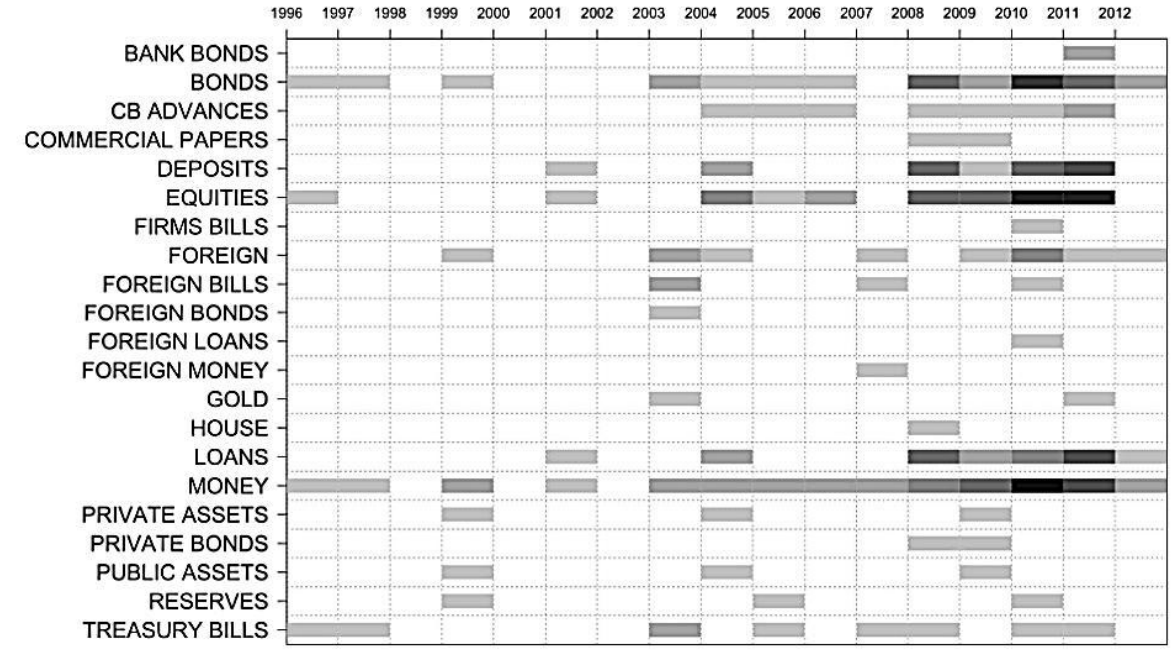
\includegraphics[width = 0.9\textwidth]{../../Escrita_Dissertacao/Da_Silveira_Dissertacao_Atual/Modelo/Caverzassi_Heatmap.png}
	\caption*{\textbf{Fonte:} \textcite[p.~4]{caverzasi_stock-flow_2013}}
\end{figure}


Uma forma de conectar o investimento residencial com o modelo do supermultiplicador sraffiano é por meio da taxa própria de juros dos imóveis (Taxa Própria) desenvolvida por \textcite{teixeira_crescimento_2015} para avaliar o caso norte americano e é definida como a taxa de juros hipotecária ($r_{mo}$) deflacionada pela inflação dos imóveis ({$\dot p_h$}) de modo que o investimento residencial, autônomo e não criador de capacidade produtiva, cresce a taxa $g_Z$ dada por:
\begin{equation}
g_Z = \phi_0 - \phi_1 \overbrace{\left(\frac{1+r_{mo}}{1+\dot p_h} - 1\right)}^{\text{Taxa Própria}}
\end{equation}
em que os $\phi_i$s são parâmetros e cujo termo em parênteses é a Taxa Própria. O primeiro parâmetro se refere aos determinantes de longo prazo (\textit{e.g.} arranjos institucionais do mercado imobiliários e de crédito) enquanto o segundo capta a demanda por imóveis decorrente das expectativas de ganhos de capital resultantes da especulação com o estoque de imóveis existente e diz respeito ao ciclo econômico.

Em outras palavras, a taxa de juros das hipotecas capta o serviço da dívida para os ``investidores'' (neste caso, famílias) enquanto a variação do preço dos imóveis permite incorporar mudança no patrimonio líquido. Portanto, aufere de modo satisfatório o custo real em imóveis de se comprar imóveis \cite[p.~53]{teixeira_crescimento_2015}. Desse modo, a partir da taxa própria de juros do imóveis é possível revelar importância do investimento residencial para além do ciclo e estendê-la para o longo prazo.  Tal proposta, portanto, lança luz sobre a influência da inflação imobiliária na construção de novos imóveis e, de acordo com o supermultiplicador sraffiano, sobre o produto como um todo. 

Como mencionado anteriormente, a referida taxa própria dos imóveis foi desenvolvida para examinar a bolha de ativos ocorria nos EUA e, portanto, não foi feita uma investigação a despeito da aplicabilidade para outros países e este é um dos objetivos desta pesquisa. Além disso, uma vez que a dívida hipotecária é o principal componente do endividamento das famílias, se faz necessária uma melhor compreensão da conexão entre o investimento residencial com as formas de financiamento e estoques financeiros de forma integrada. Nesses termos, a abordagem SFC se mostra a mais adequada para este tipo de análise. Sendo assim, um modelo de crescimento do tipo SSM com a metologia SFC (adiante, SSM-SFC) se mostra com uma alternativa para tratar do investimento residencial em que são mapeadas as relações financeiras entre os diferentes agentes institucionais.


%PERGUNTA
Compreendido este panorama, a presente investigação pretende responder a seguinte pergunta: quais os principais determinantes institucionais que explicam as especificidades do caso norte-americano frente aos demais países da OCDE a despeito das implicações macroeconômicas do investimento residencial? Como conectar o mercado imobiliário e de crédito em um modelo SSM-SFC? 
Portanto, esta pesquisa segue o caminho aberto por \textcite{brochier_supermultiplier_2018} ao adicionar um tratamento adequado das relações financeiras no SSM por meio da metodologia SFC estentendo as contribuições de: 
(i) \textcite{jorda_great_2014} ao investigar o processo de ``hipotecarização'' sob um prisma pós-keynesiano; 
(ii) \textcite{serrano_sraffian_1995} ao incluir o investimento residencial na agenda de pesquisa do supermultiplicador sraffiano; 
(iii) \textcite{teixeira_crescimento_2015} ao avaliar a aplicabilidade da taxa própria de juros para além dos Estados Unidos e;
(iv) \textcite{da_silveira_investimento_2019} ao conectar as relações entre o mercado imobiliário e de crédito diante das especificidades institucionais destacas anteriormente. 